\section{The capability--detectability frontier in full}
\label{sec:frontier-full}

Detection rates alone do not say whether a defence matters. An attacker who evades the monitor but learns nothing has not won. To weigh the two, we distilled every campaign we studied into a small student and measured what it learned.

\paragraph{Protocol.} Each campaign is turned into exactly the (prompt, answer) pairs it would collect, and a student is fine-tuned on them. For dataset prompts the answers are the dataset's; for natural prompts they are the ChatGPT replies recorded in WildChat. Capability is accuracy on GSM8K test problems \citep{cobbe2021gsm8k}. Answers come from datasets and logs, not from a live victim; Section~\ref{sec:limitations} discusses what that leaves open.

\subsection{Two regimes: elicitation and extraction}

The first measurements showed no cost of mimicry at all, and the reason turned out to be informative. A Qwen2.5-0.5B student \citep{qwen2024qwen25} gained 9.8 GSM8K points from only 100 math prompts and no more from 900; mixing in natural prompts, or restricting to natural-looking math prompts, gained as much. A larger student on a harder target (Qwen2.5-1.5B on MATH-500) behaved the same way: flat gains from 1{,}000 to 4{,}000 queries. These students already had the skill; a hundred examples teach them the answer format. We call this the \emph{elicitation} regime, in line with the finding that imitation of proprietary models transfers style far more than capability \citep{gudibande2024false}. In this regime stealth is free, and the attacker can also stay small.

A price of stealth can only appear when the student \emph{lacks} the capability, so that every useful query counts. SmolLM2-360M \citep{allal2025smollm2} solves only 3.5\% of GSM8K. Fully fine-tuned on MetaMathQA math prompts, it gained 7.5, 10.4 and 15.9 points at 1{,}000, 3{,}000 and 10{,}000 queries---the \emph{extraction} regime (Figure~\ref{fig:stealth-full}a). Here padding half of every campaign with natural prompts cost 3.6, 2.8 and 3.8 points, or 48\%, 27\% and 24\% of the gain, consistently across seeds. The natural prompts contributed nothing: a padded campaign of $n$ queries learned about as much as an unpadded campaign of $n/2$. The cost of mimicry is the queries spent on it.

\begin{figure}[t]
\centering
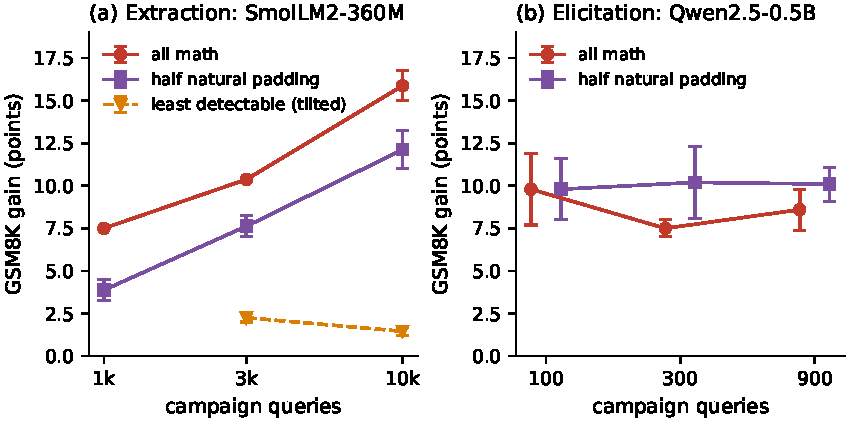
\includegraphics[width=0.85\linewidth]{figs/price_of_stealth.pdf}
\caption{The price of stealth depends on whether the student already has the skill. (a) Extraction regime: SmolLM2-360M, which starts at 3.5\% on GSM8K, keeps gaining with budget; padding half the campaign costs 3--4 points at every budget, and the least-detectable (tilted) campaign gains almost nothing (bars: range over two seeds). (b) Elicitation regime: Qwen2.5-0.5B on GSM8K (three seeds) saturates within 100 queries, and padding costs nothing measurable.}
\label{fig:stealth-full}
\end{figure}

\subsection{The covert end: campaigns that evade every detector}

Proposition~\ref{prop:lfc} says what the least-detectable campaign looks like: real benign prompts, re-weighted toward the useful region. We built it from the attacker's pool---half real WildChat prompts that a classifier places in the math region, half the rest. It evaded every detector (weekly detection at most 0.01 on development weeks, at most 0.04 on untouched weeks) and gained 2.2 points at 3{,}000 queries, against 10.4 for the dataset campaign: covertness cost 79\% of the gain.

An obvious objection is that WildChat's math questions are simply the wrong kind of math. We tested the attacker that decides the question: one that \emph{writes} its own useful prompts in the voice of real users. An instruction-tuned model (Qwen2.5-1.5B-Instruct) rewrote GSM8K-style problems as messages from WildChat users, shown real user messages as style examples and keeping each problem's answer. It could not write like users: a classifier told its rewrites from real prompts with AUC 0.98, and after two more rounds of regenerating every rewrite it caught, 0.97. Only 395 of 5{,}000 rewrites (7.9\%) passed as user-like. We then gave the attacker the best we could: resampling all rewrites to match the distribution of real on-task prompts as closely as the classifier could measure. That campaign evaded every detector and gained 4.4 points---42\% of the dataset campaign's gain, the most any covert campaign achieved. Its effective sample was only 151 distinct rewrites, each repeated about ten times.

\takeaway{The frontier, in one sentence.}{In our testbed, every campaign that evaded every detector also gave up 58--79\% of what a detectable campaign transferred, and each was limited by its supply of prompts that are both useful and indistinguishable from users'.}

This conclusion is narrower than it sounds, and we want to be explicit about how narrow. It rests on one 360M student, one benchmark, answers taken from datasets rather than a live victim, and two seeds; the student solves 14 of 400 problems at baseline, so the covert gains of 1.1--4.4 points are differences of 4--18 problems. The 213 rewrites that passed the first filter gained 3.5 points on their own, which may be format learning even in this regime. And the supply limit is exactly what attackers with a user base do not face (Section~\ref{sec:world}). A stronger writer, a live teacher and more seeds are the obvious next tests.

\subsection{Capability held at first detection}

What an attacker optimises is the capability it holds when it is first caught. Table~\ref{tab:timefrontier} combines the gain curves with detection times at the weekly campaign size of our detection experiments (1{,}640 queries a week), under two detection rules applied the same way to every detector. The \emph{first weekly alarm} at a 1\% threshold is fast but accumulates false alarms (null runs alarmed within 16 weeks a quarter of the time on untouched weeks). The \emph{anytime-valid} conformal test martingale holds the probability of any false alarm, ever, at 1\%.



Two lessons stand out. Against the two-scale and multi-outlier tests, padding on the untouched weeks bought evasion for at least a quarter of a year at a cost of a quarter to a half of the gain. Against hollowed selection it bought nothing: padded campaigns were caught in the first week. The time to an anytime-valid alarm for hollowed selection is the most important number we did not measure.
